\documentclass{article}
\usepackage[T1]{fontenc}
\usepackage{lmodern}
\usepackage{graphicx}
\usepackage{amsmath,amssymb}
\usepackage[a4paper,margin=2cm]{geometry}
\usepackage[absolute,overlay]{textpos}
\setlength{\TPHorizModule}{1mm}
\setlength{\TPVertModule}{1mm}
\usepackage[indonesian]{babel}
\usepackage{hyperref}
\setlength{\emergencystretch}{2em}
% unit: Halaman 50

\begin{document}

% === Halaman 50 (python/native) ===

Keamanan ECC

• Untuk mengenkripsi kunci AES-128 

dengan algoritma kriptografi kunci 

public, maka:

• Ukuran kunci RSA: 3072 bit

• Ukuran kunci ECC cuku 256 bit saja

• Bagaimana cara meningkatkan 

keamanan RSA?

• Tingkatkan ukuran kunci

•  Tidak Praktis? 

• Dengan ECC, pertambahan ukuran 

kunci tidak signifikan dibandingkan RSA

*) Sumber bahan: Debdeep Mukhopadhyay, Elliptic Curve Cryptography ,

 Dept of Computer Sc and Engg IIT Madras

50

% deskripsi: gambar native xref 189
\noindent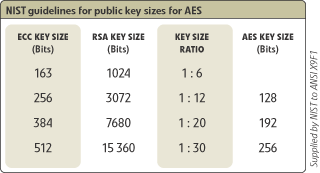
\includegraphics[width=0.85\textwidth]{../../images/python/page_050_img_01.png}

\end{document}
